\chapter{Value of the project: the influence of the number of innovation jumps}
\label{chapter:max}



%%%%%%%%%%%%%%%%%%%%%%%%%%%%%%%%%%%%%%%%%%%%%%%%%%%%%%%%%%%%%%%%%%%%%%%%
\section{Introduction}
\label{section:max_intro}

In the three previous sections we have calculated the value function associated to three different contexts (introduction of a new product; introduction of a new product with the immediate replacement of the \textit{old} one; introduction of a \textit{new} product with the possibility of immediate replacement of the \textit{old} one or simultaneous production followed by the replacement of the \textit{old} product), while considering a fixed level of innovation $\theta$.

Now we are interested to calculate the maximized expected value function, associated to each of the three contexts, with respect to the R\&D investment made and taking into account the waiting time until the desired threshold value $\theta$ is achieved.
This allows us to give a weight depending on the time we need to wait until we are able to introduce the \textit{new} product.

Here we will consider the case when $\theta$ is achieved at the next jump and, the generalization of it, when only at the $n$-th jump ($n \in \mathds{N}$) we obtain the desired threshold $\theta$.



As stated in Section \ref{intro:notation}, recall that the innovation process $\Theta=\{ \theta(t), \ t \geq 0 \}$ is defined as a Compound Poisson Process with constant rate given by $\lambda(R)=R^\gamma, \ \gamma \in (0,1)$. 
Here $R$ corresponds to the investment in the R\&D department and it is related with the size of laboratory, wages of scientists and some other aspects necessary to the research process. The higher the R\&D investment, the smaller the expected waiting time until the desired level $\theta$ occurs is, so the higher the value function will be.

Note that the investment in R\&D $R$ is different from the investment costs $\delta K$ in the sense that $R$ influences directly the innovation process $\Theta$, %allowing the research to progress faster (or slower) and thus to reach the innovation threshold desired earlier (or later),
while $\delta K$ is related with the costs that the firm needs to incur (in its factories) to adapt its production to the innovation level $\theta$, like new machines or workshops to teach workers how to use the new technology.



The innovation process can be then expressed as
$$\theta_t=\theta_0+uN_t, \ t\geq 0.$$ 
with $\theta_0$ denoting the state of technology at the initial point in time, $u>0$ is a fixed jump size and $\{ N_t, \ t \geq 0 \}$ follows a Poisson Process with rate $\lambda(R)$. 
%Note that the higher the innovation threshold $\theta$ desired, the later the innovation will occur (in average), but the higher the demand for the \textit{new} product will be.

Consider now $S_n$ as the random variable that represents the waiting time until the $n$-th jump is observed, that is,
$$S_n=\min \{t\geq 0: N(t)=n \}.$$

Accordingly to \cite{ross}, we have that $S_n$ is distributed according to Erlang distribution with shape parameter $n$ and rate parameter being the same as the Poisson Process, that is, $\lambda(R)$. From this it follows that the expected waiting time for the $n$-th jump to be reached is given by $\mathds{E}(S_n)=\frac{n}{\lambda(R)}.$ Thus, the higher the investment, the bigger the quantity of jumps observed is. Note that, in the situation in which there is no R\&D investment, there is also no evolution in the innovation process, since it implies a null rate $\lambda(0)=0$ followed by an infinite waiting time for any amount of jumps wanted to be observed.

Note from previous deduced expressions of value function that none of them depend on the R\&D investment $R$. This one only influences the innovation process. Therefore, as it will be showed in the next sections, this is a standard maximization problem, in which we will want to maximize the expected value function with respect to the R\&D investment $R$.
% the work made in the last chapter of \cite{rita}, since our investment decision is not done based on a certain optimal innovation level, but, instead, based on optimal demand level(s), only after a threshold innovation level $\theta$ is reached.

%%%%%%%%%%%%%%%%%%%%%%%%%%%%%%%%%%%%%%%%%%%%%%%%%%%%%%%%%%%%%%%%%%%%%%%%
\section{One jump}
\label{section:max_1jump}

We start with the simpler case: the desired innovation level $\theta$ is reached in the next innovation jump.
Therefore $S_1$ denotes the random variable associated to the waiting time until the jump occurs and it is such that
$$S_1 \sim \text{Erlang}(1,\lambda(R)) \overset{d}{=} \text{Exponential}(\lambda(R)).$$

We also will denote here $F$ to be the value function for a fixed situation and $V$ to be given by
\begin{equation}
	V(x)=\max_R \mathds{E} [ e^{-rS_1}F(x)-R]\geq 0
	\label{max_V}
\end{equation}
and corresponding to the maximized expected discounted value function minus the R\&D investment needed to be made. Recall that, in the previous sections, we deduced all the value functions by setting the initial time to be the time at the innovation threshold $\theta$ is reached. Therefore in order to have the real value, we need to discount it to the time when the jump happens, that is, $S_1$. Also, since the jumps are governed by a stochastic process (and thus they are random), we need to calculate the expected value of the discounted value function. Since the R\&D investment $R$ is deterministic, it could be inside or outside the expected value (but for the sake of simplicity we decided to include it when calculating the expectation).

In order to estimate the function $V$, one could have stayed just with stochastic simulations, using Monte Carlo methods for instance. However we preferred to deduce an analytical result, since its stronger than any estimation made. 

Coming back to the expression of $V$ in \eqref{max_V}, and by considering the expectation with respect to $S_1$ we obtain that it follows
\begin{align}
 V(x)&=\max_R  \left\{ \int_0 ^\infty f_{S_1}(t) e^{-rt} F(x) dt -R \right\} \nonumber \\
 &=\max_R  \left\{ \int_0 ^\infty \lambda(R) e^{-\lambda(R)t} e^{-rt} F(x) dt -R \right\} \label{max_V2}
\end{align}
where $f_{S_1}$ corresponds to the probability density function of an Exponential with parameter $\lambda(R)$, associated to the random variable $S_1$.

Since, as previously written (and deduced), none of the value functions studied depend on the R\&D investment or the time at they are evaluated, only on the demand level observed at the breakthrough, $F$ never depends on $R$ or $t$. Therefore from \eqref{max_V2}, we obtain
\begin{equation}
V(x)=\max_R \left\{ \frac{\lambda(R)}{\lambda(R)+r} F(x) -R \right\}=\max_R \left\{ \frac{R^\gamma}{R^\gamma+r} F(x) -R \right\},
\label{max_V3}
\end{equation}
which is a maximization problem with respect to the R\&D investment $R$. Since by \eqref{max_V}, $V$ is expected to be greater or equal to 0 it follows that the restriction
\begin{equation}
R^\gamma F(x) - (R^\gamma+r)R \geq 0 \ \Leftrightarrow  F(x) \geq \frac{R^\gamma+r}{R^{\gamma-1}}
	\label{max_rest}
\end{equation}
must be always verified.

The optimal value of the investment to be made, from now on denoted by $R^*$, is found by analyzing the first and the second partial derivatives of the expression to maximize, that is,
\begin{align}
\frac{\partial}{\partial R} \left( \frac{R^\gamma}{R^\gamma+r} F(x) -R \right) &= \frac{\gamma R^{\gamma-1}F(x)r-(R^\gamma+r)^2}{(R^\gamma+r)^2} \label{max_ddR}\\
\frac{\partial^2}{\partial R^2} \left( \frac{R^\gamma}{R^\gamma+r} F(x) -R \right) &=
-\frac{F(x) \gamma r R^{-2+\gamma}(r-\gamma r+(1+\gamma)R^\gamma)}{(R^\gamma+r)^3}\leq 0.
\label{max_d2dR2}
\end{align}

Note that, since $\gamma \in (0,1]$, $F(x)\geq0 \ \forall x$ and $r, \ R >0$, the second partial derivative with respect to $R$ \eqref{max_d2dR2} is always negative. Hence the expression to be maximized in \eqref{max_V3} is a concave function and we always are able to find a $R^*=\arg \underset{R}{\max} \left\{ \frac{R^\gamma}{R^\gamma+r} F(x) -R \right\}$.

Regarding the set of possible values for $\gamma$ and their interest, we consider two different cases.

Firstly we analyse the solution for $\gamma=1$, although this implies that the jump's rate is equal to $R$, it is, nevertheless, an important case since it was the only one for which we were able to obtain an analytical solution. Secondly we analyze the other possible values $\gamma \in (0,1)$, but only through a numerical solver and using software \texttt{Mathematica}.

The case $\gamma=0$ will not be considered due to its lack of importance, regarding the problem in hands. Note that $$\gamma=0 \ \Rightarrow \ \lambda(R)=1,$$
that is, considering $\gamma=0$, the innovation rate is not influenced by the size of the R\&D investment made (which is not compatible with the real life).

$\bullet$ \textbf{Case I:} $\gamma=1 \Leftrightarrow \lambda(R)=R$

Analysing the roots of the first partial derivative in order to parameter $R$, we get a quadratic polynomial for which we can calculate obtain the expression of the zeros, obtaining
%$$   \frac{\partial}{\partial R} \left( \frac{R}{R+r} F(X) -R \right) = \frac{ F(X)r-(R+r)^2}{(R+r)^2}=0 $$
%$$   \Rightarrow F(X)r-(R^2+2rR+r^2)=0$$
$$  R=-\sqrt{F(x)r}-r \  \vee \ R=\sqrt{F(x)r}-r$$

The first solution is not admissible, since it's not possible to have negative investment ($R>0$).

The second solution is admissible, if considering the restriction in \eqref{max_rest}, since we obtain
\begin{align}
 \sqrt{F(x)r}-r  \ &\underset{\eqref{max_rest}}{\geq} \ \sqrt{(R+r)r}-r \geq 0 \\
 &\Leftrightarrow rR+r^2-r^2=rR\geq 0,
 %= \sqrt{rR+R^2}-r  \ \underset{\triangle}{\geq} \ \sqrt{rR}+\sqrt{R^2}-r=\sqrt{rR},
\end{align}
which always holds since both discount rate $r$ and R\&D investment $R$ are positive.

On account of the negativity concerning the second partial derivative \eqref{max_d2dR2}, we obtain that, if \eqref{max_rest} holds, then the optimal R\&D investment to be made corresponds to
\begin{equation}
R^*=\max_R V(x)= \sqrt{F(x)r}-r.
\end{equation}


$\bullet$ \textbf{Case II:} $\gamma \in (0,1) $

Now, considering $\gamma \in (0,1) $ and taking into account expression \eqref{max_ddR}, stationary points will be found by calculating the roots of the following polynomial
\begin{equation}
R^{\gamma-1}F(x)r-R^{2\gamma}-2rR^\gamma-r^2=0.
 \label{max_root}
\end{equation}

From condition \eqref{max_d2dR2} it follows that the maximizer $R^*$ is such that it verifies \eqref{max_rest} and \eqref{max_root}.

Unfortunately, we are not able to solve \eqref{max_root} analytically for any value $\gamma \in (0,1) $. However, using software \texttt{Mathematica}, we performed some numerical illustrations for values $\gamma \in (0,1)$ presented in Section \ref{subsec:RDcap1}.


\section{Multiple jumps}
\label{section:max_jumps}

Now we generalize the context of the previous section, by considering that the desired innovation level $\theta$ is reached at the $n$-th innovation jump.
Therefore we consider $S_n$ to be the random variable associated to the waiting time until the $n$-th jump occurs and it is such that
$$S_n \sim \text{Erlang}(n,\lambda(R)).$$

By considering $n=1$, we are in situation analysed in the previous section.

For the sake of simplicity we keep the same notation as before, where $F$ denotes the value function associated to a certain investment situation and $V$ the maximized expected discounted value function minus the R\&D investment needed to be made, is now given by
\begin{align}
V_n(x)&=\max_R \mathds{E} [ e^{-rS_n}F(x)-R] \nonumber \\
&=\max_R  \left\{ \int_0 ^\infty f_{S_n}(t) e^{-rt} F(x) dt -R \right\} \nonumber \\
&=\max_R  \left\{ \int_0 ^\infty \frac{\lambda(R)^n t^{n-1}}{(n-1)!} e^{-\lambda(R)t} e^{-rt} F(x) dt -R \right\}
\label{max_2V}
\end{align}
where $f_{S_n}$ corresponds to the probability density function of an Erlang with shape parameter $n$ and rate parameter $\lambda(R)$, associated to the random variable $S_n$.

Considering $W$ to be a random variable such that $W \sim \text{Erlang}(n, \lambda(R)+r)$ and $f_W$ the correspondent probability density function, the integral above can be simplified as it follows
\begin{align}
\int_0 ^\infty \frac{\lambda(R)^n t^{n-1}}{(n-1)!} e^{-\lambda(R)t} e^{-rt} F(x) dt &=
\frac{\lambda(R)^n}{(\lambda(R)+r)^n} F(x) \int_0 ^\infty \frac{(\lambda(R)+r)^n t^{n-1}}{(n-1)!} e^{-t(\lambda(R)+r)^n)} dt \nonumber \\
&=\left( \frac{\lambda(R)}{\lambda(R)+r}\right)^n F(x)  \int_0 ^\infty f_W(t) \ dt \nonumber \\
&=\left( \frac{\lambda(R)}{\lambda(R)+r}\right)^n F(x). \label{max_2V2}
\end{align}

Plugging the resultant expression \eqref{max_2V2} in \eqref{max_2V}, we obtain that $V_n$ corresponds to a maximization problem given by
\begin{equation}
V_n(x)=\max_R \left\{ \left( \frac{\lambda(R)}{\lambda(R)+r}\right)^n F(x)-R \right\}=\max_R \left\{ \left( \frac{R^\gamma}{R^\gamma+r}\right)^n F(x)-R \right\}.
	\label{max_2V3}
\end{equation}

Since $V_n$ is expected to be greater or equal to 0 $\forall n \in \mathds{N}$, the following restriction must hold
\begin{align}
R^{\gamma n} F(x)-(R^\gamma + r)^n \geq 0 \  \Leftrightarrow \ F(x) \geq \frac{(R^\gamma+r)^n}{R^{\gamma n -1}}.
\label{max_2rest}
\end{align}


The optimal investment to be made considering that at the $n$-th jump we achieve the desired breakthrough level $\theta$, denoted by $R^*_n$, is found by analysing the first and the second partial derivatives of the expression to maximize, that is,
\begin{align}
\frac{\partial}{\partial R} \left( \left( \frac{R^\gamma}{R^\gamma+r}\right)^n F(x)-R \right) &= \frac{\gamma  F(x) n r \left(\frac{R^{\gamma }}{r+R^{\gamma }}\right)^n-r R+R^{\gamma +1}}{r R+R^{\gamma +1}} \label{max_2ddR}\\
\frac{\partial^2}{\partial R^2} \left( \left( \frac{R^\gamma}{R^\gamma+r}\right)^n F(x)-R\right) &=
\frac{\gamma  F(x) n r \left(\frac{R^{\gamma }}{r+R^{\gamma }}\right)^n \left(r (\gamma  n-1)-(\gamma +1) R^{\gamma }\right)}{R^2 \left(r+R^{\gamma }\right)^2}.
\label{max_2d2dR2}
\end{align}

This time we are not able to deduce if the second partial derivative is negative. Thus, in order to check if a stationary point is a minimum or a maximum, we will replace its value on expression \eqref{max_2d2dR2}. If it leads to a negative value, it will be considered as a relative maximum. $R^*$ will be selected among all these values to be one that maximizes the most $V_n$.

We are not even able to find any stationary point analytically, due to the complexity of \eqref{max_2ddR}.













\section{Comparative Statics}

In this Section we will check how $R^*$ and $\lambda(R^*)$ behaves with $\gamma$ and how $V_n$ behaves with $\gamma$ and $n \in \mathds{N}$.

As stated in Section \ref{section:max_jumps}, we are not able to find an analytical expression regarding the roots of expression \eqref{max_2ddR} and hence we are not able to derive ana analytical expression for the optimal R\&D investment $R^*$. However, we developed a function that, given a certain parameter $\gamma$ and an amount of jumps $n$ and considering a fixed discount rate $r$ and the value function evaluated for an initial demand level $x$ $F(x)$, calculates numerically the R\&D investment that optimizes expression \eqref{max_ddR}, that leads to function $V_n$. This function is presented in Appendix by the name \texttt{calcR}. All of the next results were obtained using it.

The following parameters were considered regarding all the next results:
\begin{itemize}
	\item $r=0.05$;
	\item $F(X)=10$;
\end{itemize}
We also considered different values of $\gamma \in (0,1]$, starting in 0.05 and, incremented by 0.05, until 1.

Note on expression \eqref{max_2V3}, since $F(x)$ is not influenced by $\gamma$ or $R$, it can be seen as a constant term representing the value of the project assuming an innovation level $\theta$, which is yet to come. Hence we are able to proceed with our numerical approximations.

We start by analysing the case when we are able to decide when to invest after a jump. That is the case when $n=1$.

\begin{figure}[!htb]
	\begin{subfigmatrix}{2}
		\subfigure[$R \in {(0,1]} $ and $\gamma \in {(0,1]} $. ]{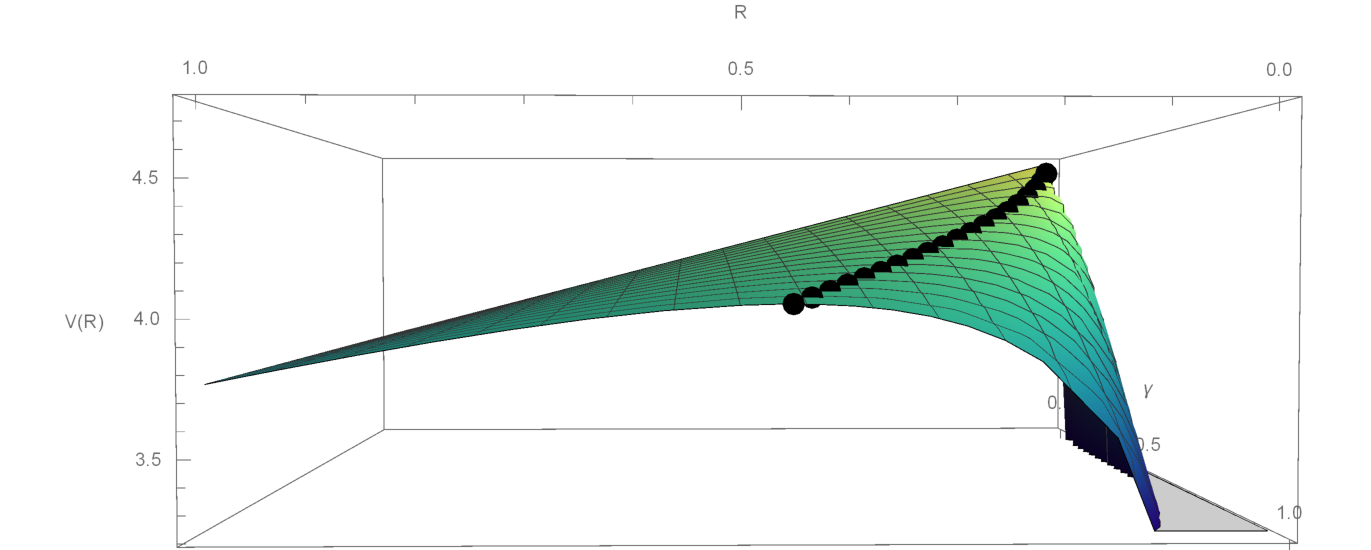
\includegraphics[width=0.45\textwidth]{Jumps/RgammaV.pdf}}
		\subfigure[A particular case: $\gamma=0.5$.
		]{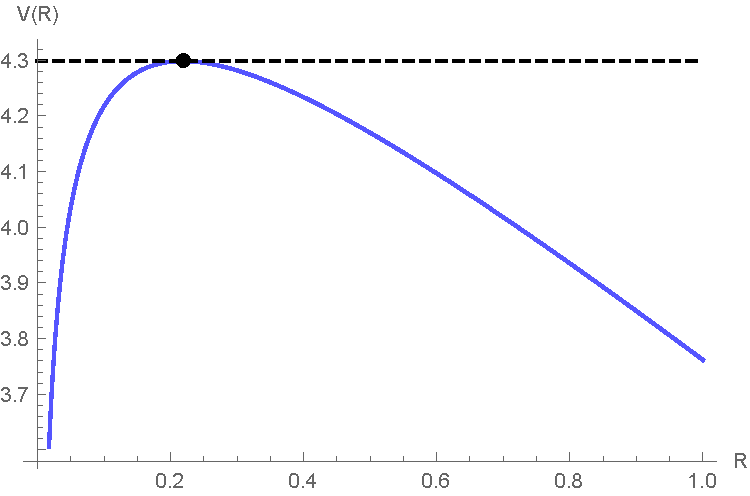
\includegraphics[width=0.45\textwidth]{Jumps/RVgamma5.pdf}}
	\end{subfigmatrix}
	\caption{Function to be maximized in \eqref{max_V} with respect to parameters $\gamma$ and $R$ and corresponding maximum values $V_1$ regarding each $\gamma$ (black)}
	\label{fig:max_n1}
\end{figure}

On the leftmost side of Figure \ref{fig:max_n1} we observe that the function to be maximized is convex regarding the R\&D investment $R$, as stated in \eqref{max_d2dR2}. Note that a smaller value of $\gamma$ implies a higher value of $R^*$. This seems to be related with the fact that a smaller $\gamma$ leads to higher jump rate, which implies a higher expected time. Thus, to balance this increasing on the expected waiting time, one increases the R\&D investment.

On the rightmost side of Figure \ref{fig:max_n1} we have the particular case when $\gamma=0.5$ and the optimal R\&D investment, calculated numerically. For $n=1$ we were able to obtain all $R^*$, but same didn't hold for bigger values of $n$ (as it will be seen in the following figures).

Now we increase the complexity and analyse the behaviour of $R^*$, $\lambda(R^*)$ e $V_n$, regarding the occurrence of 1 to 5 innovation jumps.

\begin{figure}[!htb]
	\begin{subfigmatrix}{2}
		\subfigure[3D view. ]{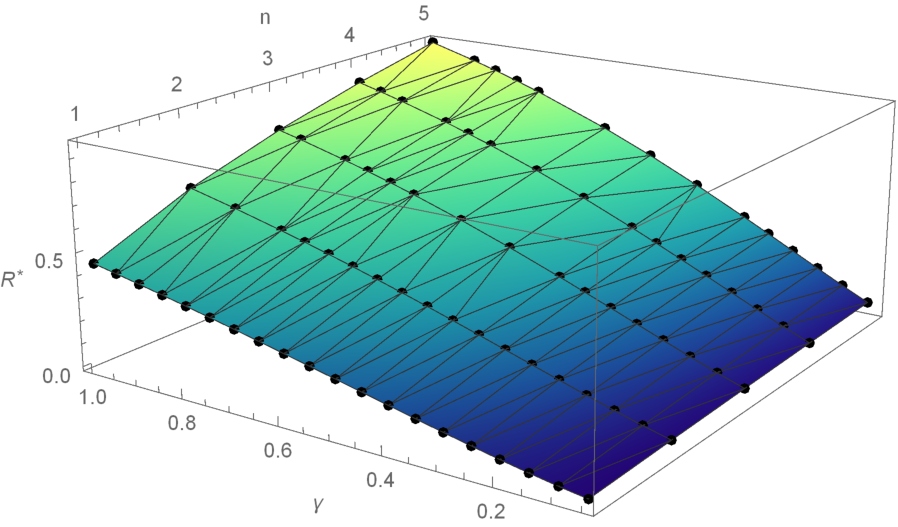
\includegraphics[width=0.45\textwidth]{Jumps/gammanR.pdf}}
		\subfigure[2D view.
		]{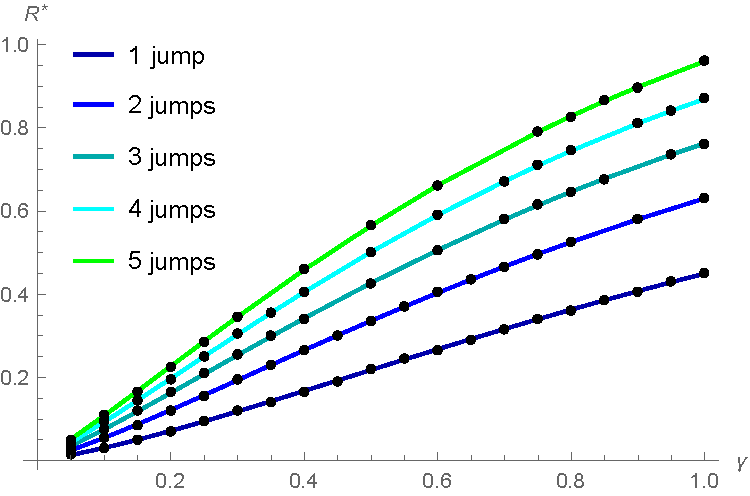
\includegraphics[width=0.45\textwidth]{Jumps/jump.pdf}}
	\end{subfigmatrix}
	\caption{Optimal R\&D values $R^*$ regarding parameter $\gamma$ and the occurrence of $n\in \{1,...,5\}$ innovation jumps with corresponding numerical approximations (black). }
	\label{fig:max_nR}
\end{figure}

On Figure \ref{fig:max_nR} one can notice that the optimal R\&D investment increases with both parameter $\gamma$ and number of jumps $n$. Note that we weren't able to obtain the optimal value $R^*$ (for instant for $\gamma=0.45$ and $\forall n\geq 3$). However by connecting the values that we were able to calculate, we are able to check the (mentioned) increasing tendency.

\begin{figure}[!htb]
	\begin{subfigmatrix}{2}
		\subfigure[Jump rate $\lambda(R^*)$. ]{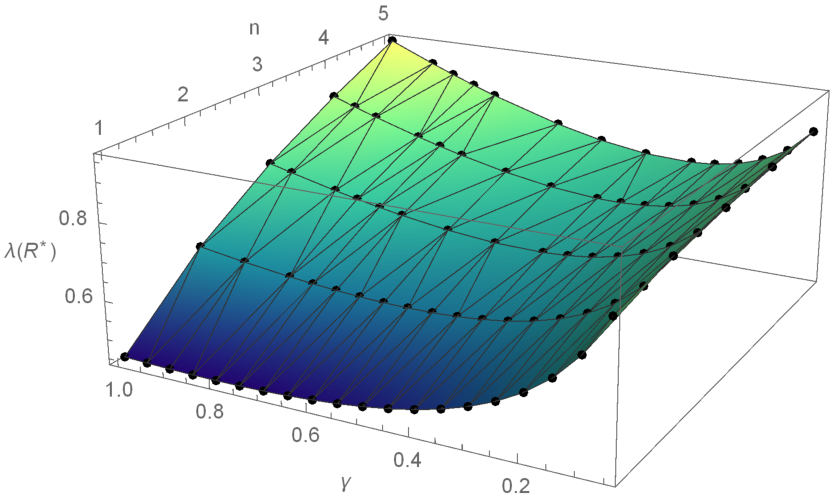
\includegraphics[width=0.45\textwidth]{Jumps/gammanlambda.pdf}}
		\subfigure[$V_n$
		]{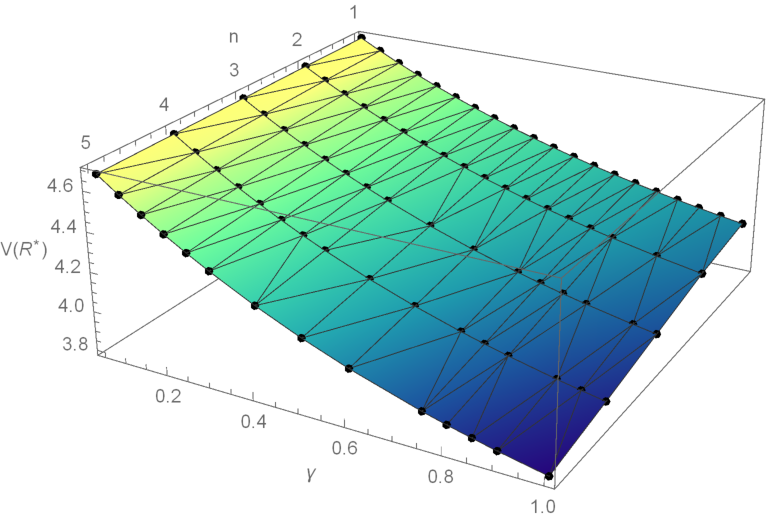
\includegraphics[width=0.45\textwidth]{Jumps/gammanV.pdf}}
	\end{subfigmatrix}
	\caption{Effect of parameters $\gamma$ and the occurrence of $n\in \{1,...,5\}$ innovation jumps on jump rate $\lambda(R^*)$ and project's value $V_n$ with corresponding numerical approximations (black). }
	\label{fig:max_n}
\end{figure}

On the leftmost side of Figure \ref{fig:max_n} one can notice that although the jump rate $\lambda(R^*)$ increases with the number of jumps considered $n$, the same doesn't hold for parameter $\gamma$ (for which it has a non-monotonic behaviour). This is related with the value $R^*$ and its exponentiation with $\gamma$, necessary to calculate $\lambda(R^*)$.

On the rightmost side of Figure \ref{fig:max_n} one can notice that the non-monotonic behaviour of $\lambda(R^*)$ seems not to influence (strongly) the tendency of $V_n$. We have that $V_n$ decreases with both $\gamma$ and $n$.
The first is explained due to the fact that if the higher the number of jumps we need to wait, before being able to think about the investment, the lower is the value of the project we have in hands (when compared with one of same value $F$ and same parameter $\gamma$).